\documentclass[12pt]{article}
\usepackage{lingmacros}
\usepackage{tree-dvips}
\usepackage{amsmath}
\usepackage{IEEEtrantools}
\usepackage{amssymb}
\usepackage{graphicx}
\usepackage{float}
\usepackage{sectsty}

\graphicspath{ {./images/} }
\sectionfont{\fontsize{16}{15}\selectfont}

\begin{document}

\begin{center}
\section*{Signal detection over an optical channel}
\end{center}
\vspace{0.5cm}
Given an optical channel, a signal on that channel can be described as a coherent state denoted by $|S\rangle$ where  $S\in\mathbb{C}$  
\newline
\newline
Considering a Noise free environment, in order to detect a signal in this type of channel, 
we use a photon counter receiver. Such a receiver is a direct detection receiver which detects 
the intensity of the optical and generates a Poisson process, where the rate of the process holds $\lambda = |S|^2$.
\newline
\newline
Suppose we have two coherent state signals denoted by $|S_0\rangle, |S_1\rangle$ and we would like to distinguish between the two 
binary hypotheses with the corresponding priori probabilities $\pi_0, \pi_1$ respectively under hypotheses $H=0,1$, 
while holding some transmission cost constraint. 
\newline
\newline
One approach was given by \textbf{Kennedy} who proposed adding a constant additional coherent state signal $|l\rangle$ 
before feeding the signal’s input to the receiver. Doing so generates a coherent state $|S+l\rangle$ which 
the receiver in turn outputs a Poisson process with rate $\lambda_i=|S_i+l|^2$.
\newline
\newline
An additional approach was given by \textbf{Dolinar} who suggested as continuation to Kennedy’s design to replace the constant 
signal with a controlled signal $|l(t)\rangle$ which is chosen adaptively based on the photon arrivals up to that moment, 
in order to achieve more certainty in the hypothesis choice with time.
\newline
\newline
The core concept of Dolinar’s updated design includes a recursive method in which the posterior probabilities of 
the two possible hypotheses denoted by $\pi_1(t), \pi_2(t)$ are updated after each step of time $\Delta$ to yield 
$\pi_1(t+\Delta), \pi_2(t+\Delta)$. 
\newline
\newline
At this point, by making $\Delta$ arbitrarily small we can expect the current Poisson process to return:
\begin{equation*}
	Poisson(\lambda) = \left\{ \,
	\begin{IEEEeqnarraybox}[][c]{l?s}
	\IEEEstrut
		0 & w.p. $(1-\lambda_i\Delta)$, \\
		1 & w.p. $(\lambda_i\Delta)$
	\IEEEstrut
	\end{IEEEeqnarraybox}
	\right.
	\label{eq:example_left_right1}
\end{equation*}
\newline
\newline
Which can be thought of as the following binary channel (Figure \ref{fig:channel}):
\newline
\pagebreak[2]
\begin{figure}[H]
  \centering
  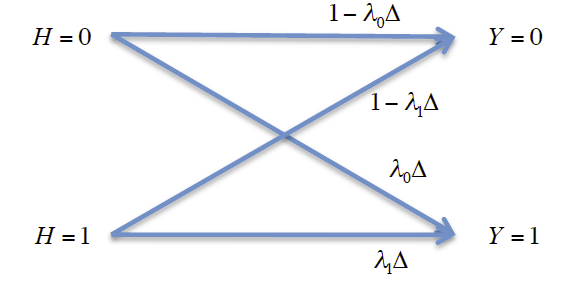
\includegraphics[width=8cm]{channel.png}
  \caption{Equivalent binary channel over time $\Delta$}
  \label{fig:channel}
\end{figure}
Since we obtained an approximation of a binary channel we may now ask how should $\l(t)$ be decided in 
other to maximize the mutual information of the binary channel.
\newline
\newline
The Entropy can be calculated as follows:
\begin{IEEEeqnarray*}{rCl}
	\IEEEeqnarraymulticol{3}{l}{
	H(Y)=H_{b}[\Delta(\pi_{0}\lambda_{0} + \pi_{1}\lambda_{1})]}
	\\*H(Y|X)=\pi_{0}H_{b}(\Delta\lambda_{1}) + \pi_{1}H_{b}(\Delta\lambda_{1})
\end{IEEEeqnarray*}
Which gives us the mutual information of the channel:
\begin{IEEEeqnarray*}{rCl}
	\IEEEeqnarraymulticol{3}{l}{
	I(X;Y)=H(Y)-H(Y|X)}
	\nonumber\\*=H_{b}[\Delta(\pi_{0}\lambda_{0} + \pi_{1}\lambda_{1})]
	\nonumber\\*\qquad\qquad-\left[\pi_{0}H_{b}(\Delta\lambda_{1}) + \pi_{1}H_{b}(\Delta\lambda_{1})\right]
	\label{eq:dont_use_multline}
\end{IEEEeqnarray*}
\pagebreak[4]
Since we want to maximize the mutual information, we shall compare its derivative to zero:
\begin{IEEEeqnarray*}{rCl}
	\IEEEeqnarraymulticol{3}{l}{
	\frac{dI(X;Y)}{dl} = 
	\log_{2}\left[\frac
		{1-\Delta[\pi_{0}\lambda_{0}+\pi_{1}\lambda_{1}]}
		{\Delta[\pi_{0}\lambda_{0}+\pi_{1}\lambda_{1}]}\right]
	2\Delta(\pi_{0}\sqrt{\lambda_{0}}+\pi_{1}\sqrt{\lambda_{1}})}
	\\*\qquad\qquad\qquad-\log_{2}\left[\frac{1-\lambda_{0}\Delta}{\lambda_{0}\Delta}\right]2\Delta\pi_{0}\sqrt{\lambda_{0}}
	\\*\qquad\qquad\qquad-\log_{2}\left[\frac{1-\lambda_{1}\Delta}{\lambda_{1}\Delta}\right]2\Delta\pi_{1}\sqrt{\lambda_{1}}
	\\*\qquad\qquad\qquad=0
\end{IEEEeqnarray*}

\begin{IEEEeqnarray*}{rCl}
	\IEEEeqnarraymulticol{3}{l}{
	\frac{dI(X;Y)}{dl} = 
	\log_{2}\left[\frac
		{1-\Delta[\pi_{0}\lambda_{0}+\pi_{1}\lambda_{1}]}
		{\Delta[\pi_{0}\lambda_{0}+\pi_{1}\lambda_{1}]}\right]
	2\Delta(\pi_{0}\sqrt{\lambda_{0}}+\pi_{1}\sqrt{\lambda_{1}})}
	\\*\qquad\qquad\qquad-2\Delta\left[\log_{2}\left(\frac{1-\lambda_{0}\Delta}{\lambda_{0}\Delta}\right)\pi_{0}\sqrt{\lambda_{0}}
	+\log_{2}\left(\frac{1-\lambda_{1}\Delta}{\lambda_{1}\Delta}\right)\pi_{1}\sqrt{\lambda_{1}}\right]
	\\*\qquad\qquad\qquad=0
\end{IEEEeqnarray*}

\end{document}